\documentclass[pmlr]{jmlr}
% OWN
\usepackage{csvsimple}
\usepackage{multirow}
\usepackage{xcolor}
\usepackage{colortbl}
\usepackage{tabu}
\usepackage[utf8]{inputenc}
\usepackage[T1]{fontenc}
\usepackage{tikz}
\usepackage{hvfloat}
\usetikzlibrary{arrows,positioning,fit,shapes,calc}

% ORIGINAL
\usepackage{rotating}% for sideways figures and tables
\usepackage{longtable}% for long tables

\usepackage{booktabs}
\usepackage[load-configurations=version-1]{siunitx} % newer version

 % The following command is just for this sample document:
\newcommand{\cs}[1]{\texttt{\char`\\#1}}

 % Define an unnumbered theorem just for this sample document:
\theorembodyfont{\upshape}
\theoremheaderfont{\scshape}
\theorempostheader{:}
\theoremsep{\newline}
\newtheorem*{note}{Note}

\usepackage[utf8]{inputenc}

 % change the arguments, as appropriate, in the following:
\jmlrvolume{1}
\jmlryear{2010}
\jmlrworkshop{Workshop Title}


% Two authors with the same address
%\author{\Name{Paweł Ksieniewicz}
%	\Email{pawel.ksieniewicz@pwr.edu.pl}\\
%	\addr 
%	Department of Systems and Computer Networks\\
%	Faculty of Electronics\\
%	Wrocław University of Science and Technology
%}
\author{\Name{--- ---}
	\Email{---}\\
	\addr 
	---\\
	---\\
	---
}

\editor{Editor's name}


\newcommand{\restable}[2] {

\scriptsize
\centering
\setlength{\tabcolsep}{3.5pt}
\def\arraystretch{1.15}
\begin{tabular}{@{}|ccccc|ccccc||ccccc|ccccc||ccc|r|}\hline%


\multicolumn{10}{|c||}{\multirow{2}{*}{\bfseries Without oversampled set}} &
\multicolumn{10}{ c||}{\multirow{2}{*}{\bfseries With oversampled set}} &
\multirow{5}{*}{\rotatebox[origin=c]{-90}{\bfseries OS}} &
\multirow{5}{*}{\rotatebox[origin=c]{-90}{\bfseries US}} &
\multirow{5}{*}{\rotatebox[origin=c]{-90}{\bfseries Full}} &
\multirow{5}{*}{\rotatebox[origin=c]{-90}{\bfseries Dataset}}
	
\\
\multicolumn{10}{|c||}{}&
\multicolumn{10}{c||}{}&
\multicolumn{3}{c|}{}&
	
	 \\
	
	\multicolumn{5}{|c|}{\bfseries Without pruning} &
	\multicolumn{5}{c||}{\bfseries With pruning} &
	\multicolumn{5}{c|}{\bfseries Without pruning} &
	\multicolumn{5}{c||}{\bfseries With pruning} 
	& & & & \\
	
	\multirow{2}{*}{\rotatebox[origin=c]{-90}{\textsc{reg}}} &
	\multirow{2}{*}{\rotatebox[origin=c]{-90}{\textsc{wei}}} &
	\multirow{2}{*}{\rotatebox[origin=c]{-90}{\textsc{con}}} &
	\multirow{2}{*}{\rotatebox[origin=c]{-90}{\textsc{nor}}} &
	\multirow{2}{*}{\rotatebox[origin=c]{-90}{\textsc{nc}}} &

	\multirow{2}{*}{\rotatebox[origin=c]{-90}{\textsc{reg}}} &
	\multirow{2}{*}{\rotatebox[origin=c]{-90}{\textsc{wei}}} &
	\multirow{2}{*}{\rotatebox[origin=c]{-90}{\textsc{con}}} &
	\multirow{2}{*}{\rotatebox[origin=c]{-90}{\textsc{nor}}} &
	\multirow{2}{*}{\rotatebox[origin=c]{-90}{\textsc{nc}}} &

	\multirow{2}{*}{\rotatebox[origin=c]{-90}{\textsc{reg}}} &
	\multirow{2}{*}{\rotatebox[origin=c]{-90}{\textsc{wei}}} &
	\multirow{2}{*}{\rotatebox[origin=c]{-90}{\textsc{con}}} &
	\multirow{2}{*}{\rotatebox[origin=c]{-90}{\textsc{nor}}} &
	\multirow{2}{*}{\rotatebox[origin=c]{-90}{\textsc{nc}}} &

	\multirow{2}{*}{\rotatebox[origin=c]{-90}{\textsc{reg}}} &
	\multirow{2}{*}{\rotatebox[origin=c]{-90}{\textsc{wei}}} &
	\multirow{2}{*}{\rotatebox[origin=c]{-90}{\textsc{con}}} &
	\multirow{2}{*}{\rotatebox[origin=c]{-90}{\textsc{nor}}} &
	\multirow{2}{*}{\rotatebox[origin=c]{-90}{\textsc{nc}}} 

	& & & &
	
	\\
	
	&&&&&&&&&&&&&&&&&&&&&&&
	\\\hline\hline
	
	\csvreader[head to column names,
	           late after line=\csvifoddrow{\\}{\\\rowcolor{gray!10!white}},
	           late after last line = \\\hline]
	{results/#1.csv}{}%
	{
	
	\ereg & \ewei & \ecwei & \enwei & \encwei &
	\eregr & \eweir & \ecweir & \enweir & \encweir &
	\eregos & \eweios & \ecweios & \enweios & \encweios & 
	\eregros & \eweiros & \ecweiros & \enweiros & \encweiros &
	\os & \us & \reg & 
	
	\multicolumn{1}{l|}{\emph{\dataset}}
	
	}%
\end{tabular}
\caption{Balanced accuracy scores obtained using #2 as a base classifier}

  
}
%TODO: Max 14 pages
%TODO: No personal information or reference to the authors should be introduced in the submitted paper.
%TODO: Submissions will be evaluated concerning their technical quality, relevance, significance, originality and clarity. 

\title
[Homogenous ensemble of undersampled majority class]
{
	Homogenous ensemble of undersampled majority class for highly imbalanced data binary classification%\titlebreak
}

\begin{document}

\maketitle

\begin{abstract}
pierwsza linia abstraktu\\
pierwsza linia abstraktu\\
pierwsza linia abstraktu\\
pierwsza linia abstraktu\\
pierwsza linia abstraktu\\
pierwsza linia abstraktu\\
pierwsza linia abstraktu\\
pierwsza linia abstraktu
\end{abstract}
\begin{keywords}
classification, classifier ensemble, undersampling, imbalanced data
\end{keywords}

%%%
%%% Introduction
%%%
\section{Introduction}
\label{sec:intro}

Most of existing classification models benefit from the assumption that there are no significant disparities between the classes of the considered problem. Nevertheless, in the real world, there are many situations in which the number of objects from one of the classes (called the \emph{majority class}) significantly exceeds the number of objects of the remaining classes (\emph{minority classes}), which often leads to decisions biased towards the \emph{majority class}. However, when considering cases such as spam filtering, medical tests or fraud detection, we may come to the conclusion that the cost of making an incorrect decision against a minority class is much greater than in other cases. The above-mentioned problem in the literature is called the \emph{imbalanced data classification} \citep{Wang:2017,Sun:2009}.

Following work focuses on the binary classification of the highly imbalanced problems, with an \textsc{ir}(\emph{imbalanced ratio}) greater than \oldstylenums{9}, which is an important issue not only in the context of the construction of appropriate models, but even a proper quality measurement \citep{Elazmeh:2006}. One of the important problems is also the fact that the number of patterns in the \emph{minority class} may be so small that it will not allow to achieve the appropriate discriminatory power of the model, which may lead to its \emph{overfitting} \citep{Chen:2008}. Most of these problems are the subject of extensive research \citep{Bunkhumpornpat:2009,Chawla:2002}.

One of the possible approaches to solve such problems are \emph{inbuild mechanisms}, trying to adapt existing classification models to balance the accuracy between classes. Popular here is the learning approach without counter-examples, using \emph{one-class classification} \citep{Japkowicz:1995, Krawczyk:2014ins}, where the aim is to get to know the decision boundaries within minority classes. The solution may also be the \emph{cost sensitive solutions}, assuming the asymmetric loss function \citep{Lopez:2012,He:2009}.

Another approach, more connected with the following paper, is the group of \emph{data preprocessing methods}, which focuses on reducing the number of majority class objects (\emph{undersampling}) or generating patterns of minority class (\emph{oversampling}) to balance a dataset. Overview of methods from this group is presented in Figure \ref{fig:preproc}. 

\begin{figure}[!h]
\floatconts
  {fig:preproc}
  {\caption{Examples of data preprocessing methods.}}
  {%
    \subfigure[Original dataset]{\label{fig:overs}%
    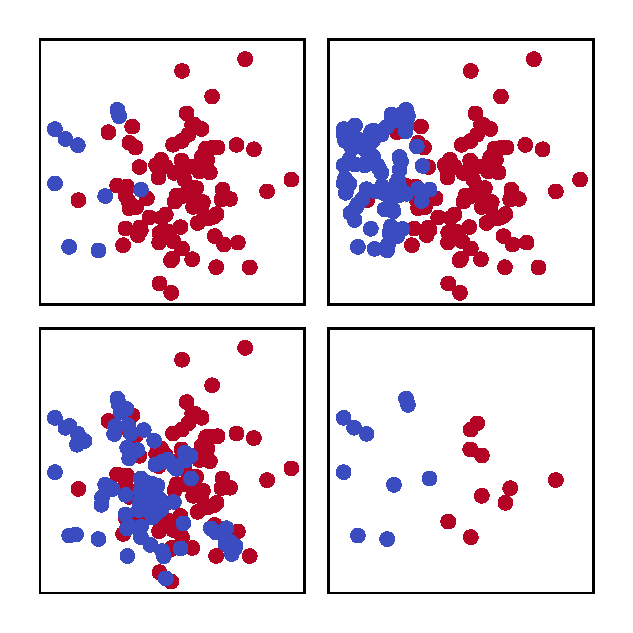
\includegraphics[clip=true, width=.25\linewidth,
    				 trim = 11 141 141 11]
    {figures/preprocessing}}%
    \qquad
    \subfigure[\textsc{smote}]{\label{fig:smote}%
    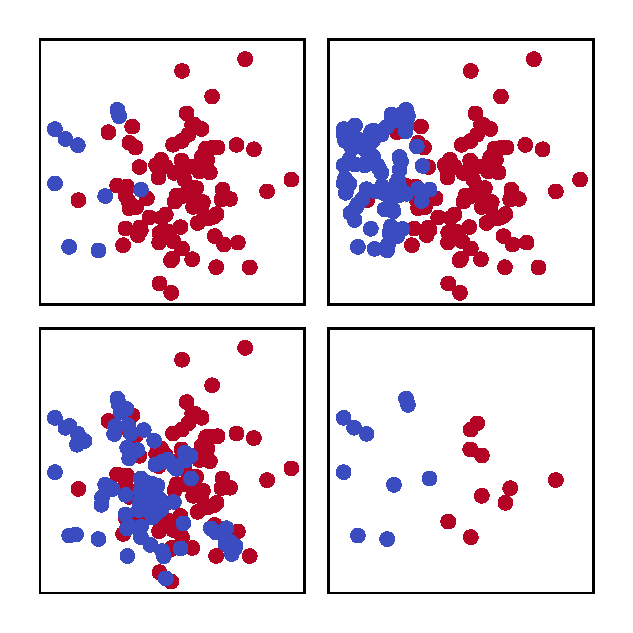
\includegraphics[clip=true, width=.25\linewidth,
    				 trim = 141 141 11 11]
    {figures/preprocessing}}%
      
    \subfigure[\textsc{adasyn}]{\label{fig:adasyn}%
    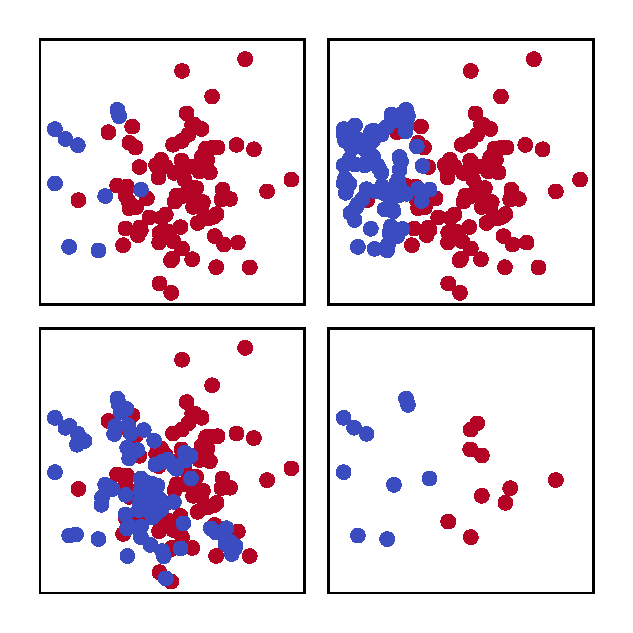
\includegraphics[clip=true, width=.25\linewidth,
    				 trim = 11 11 141 141]
    {figures/preprocessing}}%
    \qquad
    \subfigure[Undersampling]{\label{fig:unders}%
    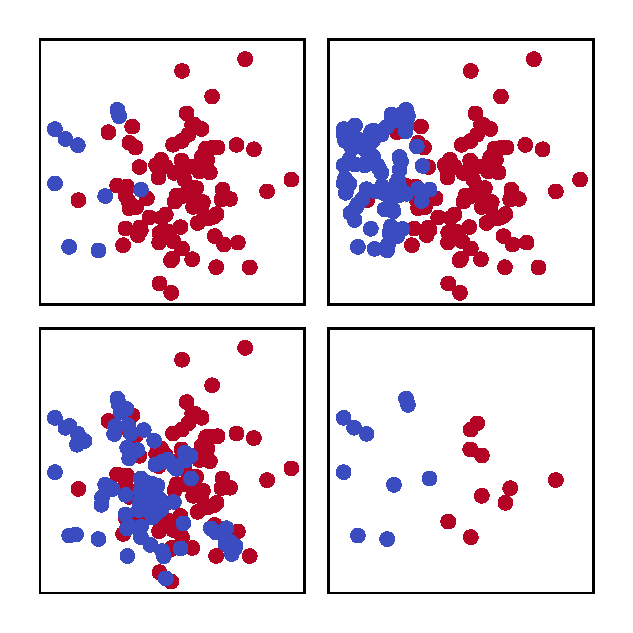
\includegraphics[clip=true, width=.25\linewidth,
    				 trim = 141 11 11 141]
    {figures/preprocessing}}%
  }
\end{figure}

These algorithms are addressing the task of balancing the number of objects within the problem classes. In the case of basic \emph{oversampling}, new objects are created as random copies of those already existing in the training set\footnote{Since the characteristics of the new patterns will be identical to those already present in the dataset, we can consider Figure \ref{fig:overs}, an illustration of the original dataset, also as the presentation of pattern distribution after oversampling.}. Currently, the most common kind of \emph{oversampling}  is \textsc{smote} \citep{Cha2002}, shown in Figure \ref{fig:smote}, creating new, synthetic objects based on $k$ averaged examples nearest to a random points from the space occupied by a minority class. An active version of \textsc{smote} is the \textsc{adasyn} algorithm \citep{He:2008}, shown in Figure \ref{fig:adasyn}, which takes into account the difficulty of synthetic samples. This approach allows to solve the problem of repeating samples in the training set, but can also lead to \emph{overfitting}, which is presented in Figure \ref{fig:wrongsmote}.

\begin{figure}[htbp]
\floatconts
  {fig:wrongsmote}
  {\caption{Example of wrong \textsc{smote} oversampling.}}
  {%
    \subfigure[Original dataset]{\label{fig:circle}%
    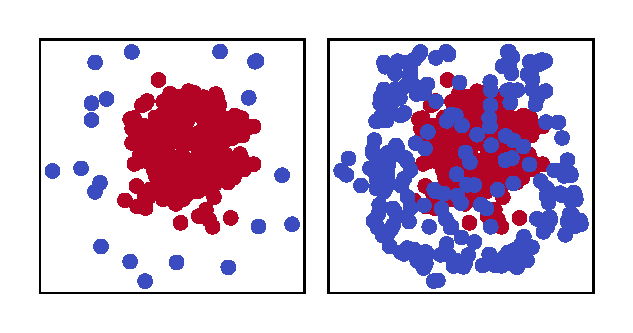
\includegraphics[clip=true, width=.25\linewidth,
    				 trim = 11 11 141 11]
    {figures/wrong_smote}}%
    \qquad
    \subfigure[\textsc{smote}]{\label{fig:circle}%
    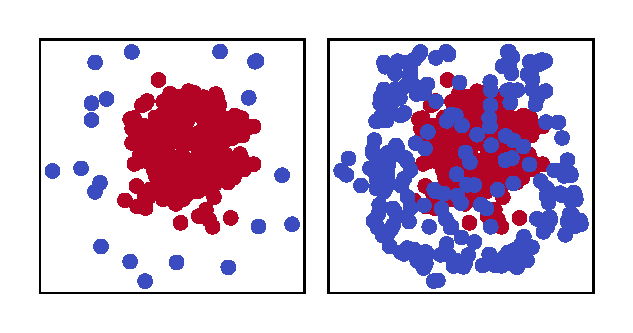
\includegraphics[clip=true, width=.25\linewidth,
    				 trim = 141 11 11 11]
    {figures/wrong_smote}}%
  }
\end{figure}

In the case of \emph{undersampling}, shown in Figure \ref{fig:unders}, in which we draw as many objects from the majority class as in the minority class, there is no risk of erroneous mixing of the distribution of classes.

The last group of methods to be mentioned are \emph{hybrid approaches}, combining \emph{over-} and \emph{undersampling} algorithms with \emph{ensemble classifiers} \citep{Galar:2012}. The \emph{Bagging} and \emph{Boosting} variants, such as \emph{AdaBoost.NC} \citep{Wang:2010} or \emph {SMOTEBoost} \citep{Chawla:2003}, have become particularly popular in this area.

The main contributions of this work are:
\begin{itemize}
	\item a method of establishing a homogenous ensemble using a \emph{k-fold undersampling} of majority class,
	\item proposition of five fusers to generate ensemble decision,
	\item a pruning method adjusting the decision rule to the \emph{testing set},
	\item implementation and experimental evaluation of proposed method.
\end{itemize}

%%%
%%% Method
%%%
\section{Homogenous ensemble based on undersampling the majority class}
\label{sec:intro}
\subsection{Establishing ensemble}

Complex oversampling methods, such as \textsc{smote} or \textsc{adasyn}, despite the large possibilities in most of the imbalanced problems, are not applicable to extreme situations where the minority class is represented by only a few samples, which makes it impossible to designate the nearest neighbors to create a new synthetic object. This could lead to the use of \emph{undersampling} in such problems, but it is characterized, due to high randomness, by a strong instability in a situation of high \textsc{ir} (\emph{imbalance ratio}), which does not allow for the development of a reliable solution.

A popular answer to the above-mentioned problem are the ensemble methods of \emph{Bagging} or \emph{Boosting}, characterized by random sampling with replacement of the training set, breaking a large problem, into a set of smaller problems. This work proposes a basic method, which also breaks the imbalanced task, but with ensuring the use of all the patterns available in the data set, but without a risk of overlapping. Its description can be found in Algorithm 1.

\begin{algorithm}[!h]
\caption{Training classifier ensemble from multiple balanced training datasets separated from one imbalanced dataset of binary problem}\label{alg:moore}
Given a dataset $DS$:
\begin{enumerate*}
	\item Divide $DS$ into subsets of minority- $MinC$ and majority-class $MajC$
	\item Calculate imbalanced ratio $IR$ as the proportion of the number of patterns in $MinC$ and $MajC$ 
	\item Establish $k$ by rounding $IR$ to nearest integer
	\item Perform a \emph{shuffled k-fold division} of $MajC$ to produce a set of subsets $MajC_1, MajC_2, \ldots, MajC_k$ 
	\item For every $i$ in range to $k$
	\begin{enumerate*}
		\item Join $MajC_i$ with $MinC$ to prepare a training set $TS_i$,
		\item Train classifier $\Psi_i$ on $TS_i$ and add it into ensemble
	\end{enumerate*}
\end{enumerate*}
\end{algorithm}

After dividing the dataset with imbalanced binary problem into separated minority ($MinC$) and majority class ($MajC$), we are calculating the \textsc{ir} (\emph{imbalanced ratio}) between given classes. Rounding \textsc{ir} to the nearest integer value $k$ allows us to find the optimal division coefficient of the majority class samples in the context of maximizing the balance between the $MinC$ and any $MajC_i$ subsets while ensuring that all $MajC$ patterns are used in learning process with no overlapping between the individual $MajC_i$'s. Each of $k$ classifiers $\Psi_i$ is trained on union of $MinC$ and $MajC_i$ sets.

\paragraph{Extending pool with oversampling} As an extension of the method of classifier ensemble construction, it is also proposed to extend its pool by a model learned on an additional data set, which is a full set of data subjected to \emph{oversampling}. It is worth testing if the knowledge gained from this method may be a valuable contribution to the ensemble decision. Due to impossibility to use \textsc{smote} or \textsc{adasyn} for oversampling the minority class with only few instances, only its basic variant will be used. 

%%% Fuser
\subsection{Fuser design}

In addition to ensuring the diversity of the classifiers pool, which we achieve by a homogenous committee built on disjoint subsets of the majority class supplemented by minority patterns, the key aspect of the hybrid classification system is the appropriate design of its \emph{fuser} -- the element responsible for making decisions based on the answers of the base classifiers.

There are two groups of solutions here. The first are based on component \emph{decisions} of the committee, most often employing the \emph{majority voting} to produce a final decision. The decision rules proposed in this work are, however, part of the second group, where the \emph{fuser} is carried out by \emph{averaging} (or \emph{accumulating}) the \emph{support vectors} received from the members of a pool.

\begin{note}
It should be remembered that in such methods, it is necessary to use a \emph{probabilistic classification model}, which also requires \emph{quantitative} and not \emph{qualitative data}.
\end{note}


Five fusers were proposed:

\begin{enumerate}
	\item \textbf{\textsc{reg}} --- regular accumulation of support.

A basic method without weighing the members of a committee.

	\item \textbf{\textsc{wei}} --- accumulation weighted after members of a committee.

The weight of the classifier in the pool is its quality achieved for the training set. We can not use here the measure of \emph{accuracy}, which does not fit with the task of the imbalanced classification, so we decided on a \emph{balanced accuracy} \citep{brodersen2010balanced}.

	\item \textbf{\textsc{nor}} --- same as \textbf{\textsc{wei}}, but with normalization of weights,

To reward classifiers with a higher \emph{discriminative power}, weights are subjected to normalization by a \emph{MinMaxScaler}.
	
	\item \textbf{\textsc{con}} --- accumulation weighted by tested patterns.
	
In order to reward classifiers with greater \emph{"certainty"} for given object, the decision for each pattern is weighted by the absolute difference between class support, for the needs of research called the \emph{contrast}. Individual classifiers in the pool do not have to be better or worse for each of the tested patterns. This is illustrated in Figure \ref{fig:contrast}, where we can see two cases of ensembles. There are tested patterns on the X axis and classifiers in the pool on the Y axis. A white square means the \emph{contrast} of 1, and therefore a \emph{sure} decision, and the black square the \emph{contrast} of 0, which describes the pattern that is exactly on the decision boundary.
	
\begin{figure}[!h]
\floatconts
  {fig:contrast}
  {\caption{Illustration of the \emph{contrast} in committees built on two different datasets.}}
  {%
    \subfigure[Example of a \emph{"sure"} ensemble]{\label{fig:circle}%
    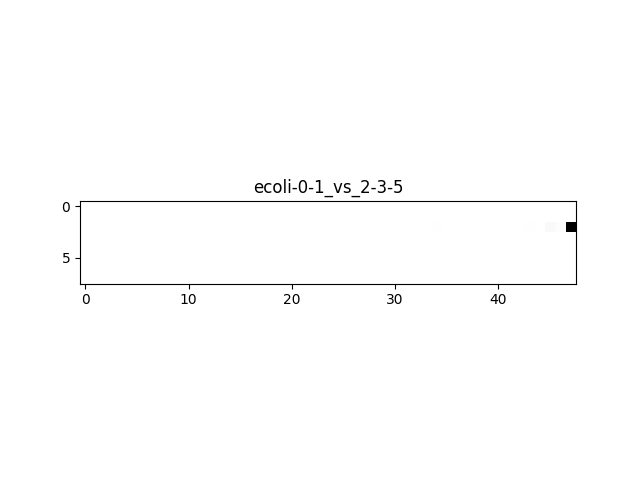
\includegraphics[width=.5\linewidth, trim = 0 100 0 100,clip=true]
    {figures/ecoli-0-1_vs_2-3-5}}%
    \subfigure[Example of \emph{"unsure"} ensemble]{\label{fig:circle}%
    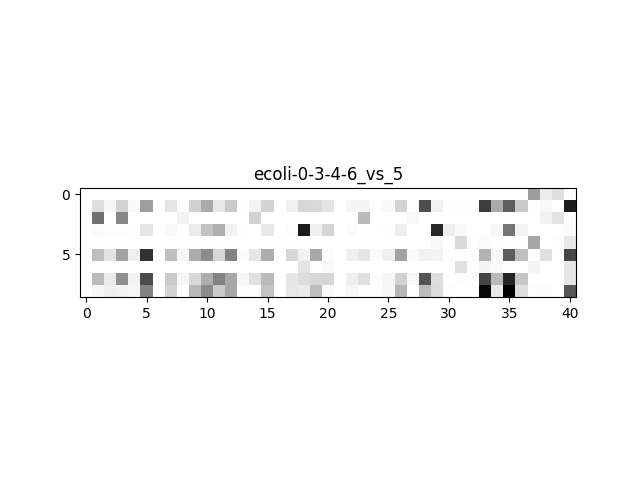
\includegraphics[width=.5\linewidth, trim = 0 100 0 100,clip=true]
    {figures/ecoli-0-3-4-6_vs_5}}%
  }
\end{figure}

	
	\item \textbf{\textsc{nci}} --- accumulation by a product of normalized weights \textbf{\textsc{nor}} and a \emph{contrast} \textbf{\textsc{con}}.
\end{enumerate}

The proposed method of constructing the committee makes its size directly dependent on the \textsc{ir}, which, given the highly unbalanced data (for example with \textsc{ir} greater than 40), leads to the construction of an extensive hybrid model. Therefore, the method of prunning it to a smaller size was also considered.

%%% Pruning
\subsection{Ensemble pruning}

In typical methods of \emph{ensemble pruning}, it follows the phase of training the committee, for example, by eliminating the classifiers that achieve the lowest quality on the \emph{training} or separated \emph{validation set}. This paper proposes a method of \emph{response pruning} based on the assumption that during the testing phase we analyze not just a single test pattern, but the entire \emph{testing set}.

\begin{figure}[!h]
\floatconts
  {fig:scheme}
  {\caption{Scheme of using k-Fold division in ensemble construction}}
  {\begin{tikzpicture}%[font=\sffamily\small]
\tikzset{el/.style={draw, rectangle, minimum width = 1cm, minimum height=1cm}}

%\draw[step=.5cm,gray!30!white,very thin] (-4,-13) grid (7,1.5);

\node[rectangle, fill=red!10!white, minimum width=3cm, minimum height=8cm]
 at (5,-3) {};

% Original training set with division
\node[el, minimum width=6cm](its) at (0,0) {Imbalanced training set};
\node[el, text width=.75cm] (minc) at (-2.5, -1.5) {\tiny $MinC$};
\node[el, minimum width = 4.5cm] (majc) at (.75, -1.5) {\tiny $MajC$};

% Pre-methods
\node[el, thick, minimum width = 4.5cm, minimum height = .5cm, rounded corners=2mm] (kfold) at (.75, -2.5)
{\scriptsize \textsc{shuffled k-fold division}};
\node[el, thick, minimum width = 2cm, minimum height = .5cm, rounded corners=2mm] (oversampling) at (5, -2.5)
{\tiny \textsc{oversampling}};

% Processed training sets
\node[el, text width=.75cm] (majc0) at (-1, -3.5) {\tiny$MajC_0$};
\node[el, text width=.75cm] (majc1) at (.5, -3.5) {\tiny$MajC_1$};
\node[el, text width=.75cm] (majck) at (2.5, -3.5) {\tiny$MajC_k$};
\node[el, text width=.75cm] (minc0) at (-1, -4.5) {\tiny$MinC$};
\node[el, text width=.75cm] (minc1) at (.5, -4.5) {\tiny$MinC$};
\node[el, text width=.75cm] (minck) at (2.5, -4.5) {\tiny$MinC$};
\node[text width = 1cm] at (1.65,-4)
{\bfseries . . .};


\node[el, minimum width = 2cm, minimum height=2cm, text width=1.75cm] (osts) at (5, -4)
{\scriptsize Oversampled training set};

% Member classifiers
\node[el, rounded corners=5mm] (c0) at (-1, -6) {$\Psi_1$};
\node[el, rounded corners=5mm] (c1) at (.5, -6) {$\Psi_2$};
\node[el, rounded corners=5mm] (ck) at (2.5, -6) {$\Psi_k$};
\node[el, minimum width=2cm, rounded corners=5mm] (co) at (5, -6) {$\Psi_{os}$};

\node[text width = 1cm] at (1.65,-6)
{\bfseries . . .};


% Testing
\node[el, minimum width=7.5cm](testset) at (2.25,-8) {Testing set};

\node[el] (s0) at (-1, -9.5) {$s_1$};
\node[el] (s1) at (.5, -9.5) {$s_2$};
\node[el] (sk) at (2.5, -9.5) {$s_k$};
\node[el, minimum width=2cm] (so) at (5, -9.5) {$s_{os}$};
\node[text width = 1cm] at (1.65,-9.5)
{\bfseries . . .};


\node[el, minimum width=7.5cm, minimum height = .5, thick, rounded corners=2mm](fuser) at (2.25,-10.75)
{\textsc{fuser}};

\node[el, minimum width=7.5cm](dec) at (2.25,-11.75)
{Decisions};


% Lines and sections
\draw [dashed] (3.5,1) -- (3.5,-7);
\node[text width = 2.75cm] at (5,.5)
{\tiny \bfseries Extending pool with oversampling};
\node[text width = 2cm] at (-2.25,-6.75)
{\tiny \bfseries Learning};
\node[text width = 2cm] at (-2.25,-7.25)
{\tiny \bfseries Classification};

\draw [dashed] (-3.5,-7) -- (6.5,-7);

% Connections
\draw[->] (its) -| (oversampling);
\draw[->] (-2.5,-.5) -- (minc);
\draw[->] (.75,-.5) -- (majc);
\draw[->] (majc) -- (kfold);

\draw[->] (-1,-2.75) -- (majc0);
\draw[->] (.5,-2.75) -- (majc1);
\draw[->] (2.5,-2.75) -- (majck);

\draw[->] (minc.south) |- (minc0.west);
\draw[<->] (minc0) -- (minc1);
\draw[<->] (minc1) -- (minck);


\draw[->] (oversampling) -- (osts);

\draw[->] (minc0) -- (c0);
\draw[->] (minc1) -- (c1);
\draw[->] (minck) -- (ck);
\draw[->] (osts) -- (co);

\draw[->] (c0) -- (-1,-7.5);
\draw[->] (c1) -- (.5,-7.5);
\draw[->] (ck) -- (2.5,-7.5);
\draw[->] (co) -- (5,-7.5);

\draw[->] (-1,-8.5) -- (s0);
\draw[->] (.5,-8.5) -- (s1);
\draw[->] (2.5,-8.5) -- (sk);
\draw[->] (5,-8.5) -- (so);

\draw[->] (s0) -- (-1,-10.5);
\draw[->] (s1) -- (.5,-10.5);
\draw[->] (sk) -- (2.5,-10.5);
\draw[->] (so) -- (5,-10.5);
\draw[->] (fuser) -- (dec);



\end{tikzpicture}
}
\end{figure}

Ensemble, receiving a \emph{testing set}, generates \emph{support vectors} ($s_i$) for each classified object, so, with a binary problem, we can treat received support for one of the problem classes as values from the \emph{random variables} to analyze their mutual statistical dependence.

In the proposed method, using the signed-rank test, we are \emph{clustering} the pool of $k$ (or $k+1$ on the \emph{oversampling} variation of a method) classifiers to $n$ groups (where $n\leq k$), to average the support and weight classes within groups to create a new set of supports from $s'_1$ to $s'_n$, passed later on to \emph{fuser}.

The scheme of the full decision model of the proposed method is shown in Figure \ref{fig:scheme}.

\begin{note}
In the considered case of pruning, we ignore the possible situation in which the answer $\Psi_1$ is dependent on $\Psi_2$, the answer $\Psi_2$ is dependent on $ \Psi_3$, but $\Psi_1$ is not dependent on $\Psi_3$. This is an interesting issue that will be addressed in future research, but to simplify the proposal, a simplified approach has been used.
\end{note}

%%%
%%% Experiment design
%%%
\section{Experiment design}
\label{sec:intro}

For the experimental evaluation of the proposed method, a collection of datasets made available with \textsc{keel} \citep{alcala2011keel} was used, focusing on a section containing highly unbalanced data, with \textsc{ir} greater than 9 \citep{fernandez2009hierarchical}. From among the available datasets, \oldstylenums{40} were selected presenting only binary problems with quantitative attributes. A review of selected datasets, including information on their number of features, the number of patterns in each class and the unbalance ratio is presented in Table \ref{tab:datasets}.


\begin{table}[!h]
%\vspace{-.5em}
\centering
\rotatebox{90}{
\scriptsize
\centering
\setlength{\tabcolsep}{3.5pt}
\def\arraystretch{1.1}
\begin{tabular}{@{}|c|ccc|c|l|@{}}\hline%

\multirow{2}{*}{\rotatebox[origin=c]{-90}{\bfseries \textsc{ir}}} &
\multicolumn{3}{c|}{\bfseries Samples} &
\multirow{2}{*}{\bfseries Features} &
\multicolumn{1}{c|}{\multirow{2}{*}{\rotatebox[origin=c]{-90}{\bfseries DS}}}
\\

&
\multicolumn{1}{c}{\textsc{all}} & 
\multicolumn{1}{c}{\textsc{maj}} & 
\multicolumn{1}{c|}{\textsc{min}} &
& 

	\\\hline\hline
	
	\csvreader[head to column names,
	           late after line=\csvifoddrow{\\}{\\\rowcolor{gray!10!white}},
	           late after last line = \\\hline]
	{results/datasets.csv}{}%
	{
	
	\ir &
	\multicolumn{1}{c}{\samples} & 
	\multicolumn{1}{c}{\majority} & 
	\multicolumn{1}{c|}{\minority} & 
	\features & 
	\multicolumn{1}{l|}{\emph{\dbname}}
		
	}%
\end{tabular}}
\caption{Summary of imbalanced datasets chosen for evaluation}\label{tab:datasets}
\end{table}
  

As may be observed in the summary, the experiments are based on datasets with relatively small spatiality (up to \oldstylenums{13} dimensions), with imbalance ratio from \oldstylenums9 to even \oldstylenums{40}. The datasets provided by \textsc{keel}, to ensure easy comparison between results presented in various research, are already pre-divided into five parts, which forces the use of \emph{k-fold cross-validation} with $k = 5$ in experiments \citep{alpaydin2009introduction}.

In the task of imbalanced data classification, due to its strong bias towards majority class, the \emph{accuracy} measure is not a proper tool. For a reliable result, a measure of \emph{balanced accuracy} is given as test results.

Both the implementation of the proposed method and the experimental environment have been constructed using the \emph{scikit-learn} library \citep{scikit-learn} in version \emph{0.20.dev0}\footnote{At the time of conducting research, only the development version of the package already has the implementation of \emph{balanced accuracy} measure.}. Among the available classification models, the \textsc{mlp} (\emph{Multilayer Perceptron}) and \textsc{svc} (\emph{Support Vector Machine}) were rejected. First one was not able to build a correct model due to the lack of convergence on the small datasets (minority class of data chosen for experiments is often represented by only two patterns in cross-validated folds) and second, whose probabilistic interpretation is measurable only with sufficiently large data sets, did not allow credible construction of a fuser. As base classifiers, the following algorithms were used:

\begin{itemize}
	\item \emph{Gaussian Naive Bayes} (\textsc{gnb}) \citep{gnb},
	%\item \emph{k-Nearest Neighbors} (k\textsc{nn}) --- with \oldstylenums{5} neighbors and \emph{Minkowski} metric,
	\item \emph{Decision Tree Classifier} (\textsc{dtc}) --- with \emph{Gini} criterion \citep{loh2011classification}.
\end{itemize}

To provide a comparative result for the method presented in the following paper, each base classifier was also tested for the raw, imbalanced dataset and its under- and oversampled versions. Undersampling, due to high instability of results, was repeated five times on each fold. Used statistical analysis tool was a paired dependency between the classifier, which achieved the highest result and each of the others, calculated using the signed-rank \emph{Wilcoxon} test \citep{wilcoxon1945individual}.

The full implementation of the proposed method and the script allowing the repetition of the presented research may be found in the git repository available at \url{url-removed-due-to-} \url{blind-review}.

%%%
%%% Introduction
%%%
\section{Experimental evaluation}
\label{sec:intro}

Przedstawienie tabel.

\begin{sidewaystable}
	\restable{GNB}{\textsc{gnb}}
\end{sidewaystable}

%\begin{sidewaystable}
%	\restable{kNN}{k\textsc{nn}}
%\end{sidewaystable}

\begin{sidewaystable}
	\restable{DTC}{\textsc{dtc}}
\end{sidewaystable}

Tabela zbiorcza zwycięstw w zależności od parametrów (z grupowaniem).


\begin{table}[!h]
%\vspace{-.5em}
\centering
\centering
\setlength{\tabcolsep}{3.5pt}
\def\arraystretch{1.1}
\begin{tabular}{@{}|c|ccc|cc|cc|ccccc|@{}}\hline%
clf & full & us & os & notos & wos & nopru & wpru & reg & wei & con & nor & nci\\\hline

%\multirow{2}{*}{\rotatebox[origin=c]{-90}{\bfseries \textsc{ir}}} &
%\multicolumn{3}{c|}{\bfseries Samples} &
%\multirow{2}{*}{\bfseries Features} &
%\multicolumn{1}{c|}{\multirow{2}{*}{\rotatebox[origin=c]{-90}{\bfseries DS}}}
%\\

%&
%\multicolumn{1}{c}{\textsc{all}} & 
%\multicolumn{1}{c}{\textsc{maj}} & 
%\multicolumn{1}{c|}{\textsc{min}} &
%& 

%	\\\hline\hline
	
	\csvreader[head to column names,
	           late after line=\csvifoddrow{\\}{\\\rowcolor{gray!10!white}},
	           late after last line = \\\hline]
	{results/summary.csv}{}%
	{\clf &
	\full & \us & \os &
	\withoutos & \withos & 
	\withoutpru & \withpru &
	\reg & \wei & \con & \nor & \nci
			
	}%
\end{tabular}
\caption{NAZWIJŻE TABELĘ}\label{tab:summary}
\end{table}

Interpretacja wyników, czyli co zostało należycie uprawdopodobnione.

%%%
%%% Conclusions
%%%
\section{Conclusions}
\label{sec:intro}
Co zostało zaproponowane.

Na co pozwala taka metoda.

Do jakich rezultatów doprowadziła.

Jakie są plany na przyszłość (czyli co robisz w wakacje).



%%%
%%% Acknowledgements and references
%%%
\acks{
	Acknowledgements go here.
}
\bibliography{bibliography}

\end{document}
